\chapter{无监督学习}

第 2 章至第 9 章详细讲解了监督学习的流程。在这些章节中,我们定义了模型,这些模型能将观测数据 x 映射到输出值 y,并引入了损失函数来衡量这种映射对于训练数据集 \({x_i , y_i }\) 的准确性。随后,我们讨论了如何对这些模型进行拟合及评估其性能。第 10 章到第 13 章则引入了采用参数共享和支持并行计算路径的更为复杂的模型架构。

无监督学习模型的核心特点在于,它们是在没有标签的情况下,从观察数据集 \({x_i}\) 学习得到的。所有的无监督模型都有这一共同点,但它们的目标却各不相同。这些模型可以用来生成数据集中的新样本,或者对样本进行操作、去噪、插值和压缩。它们还能够揭示数据集的内在结构(例如,通过把数据集分成几个有内在联系的群体)或者判断新样本是属于原有数据集还是异常值。

本章将介绍无监督学习模型的系统分类,并探讨模型理想的属性及其性能评估方法。紧接着的四章将分别深入讨论四种特殊模型:生成对抗网络(GANs)、变分自编码器(VAEs)、归一化流(Normalizing Flows)和扩散模型(Diffusion Models)。在此之前,大部分相关的数学知识都已在文中提及。但是,后续四章需要对概率学有深入的理解,附录 C 提供了所需的相关背景知识。

\section{无监督学习模型的分类}
在无监督学习的一个常见策略中,我们定义了数据示例 x 与一组未见的潜变量 z 之间的映射关系。这些潜变量揭示了数据集的底层结构,它们的维度通常低于原始数据;因此,潜变量 z 可以看作是捕获了数据示例 x 核心特征的压缩版(图 1.9-1.10)。

从原理上讲,观测变量与潜变量之间的映射可以是任一方向。有的模型将数据 x 映射到潜变量 z。例如,著名的 k-means(k-均值)算法就是将数据 x 映射到一个聚类分配 \(z \in {1,2,...,K}\)。而其他模型则是从潜变量 z 映射回数据 x。在这些模型中,定义了潜变量 z 上的分布 Pr(z)。通过 (i) 抽取该分布的样本及 (ii) 将样本映射到数据空间 x,现在可以生成新的数据示例。因此,这些模型被称为生成模型(见图 14.1)。

第 15 至 18 章介绍的四种模型都是利用潜变量的生成模型。生成对抗网络(Generative Adversarial Networks,GANs,第 15 章)通过使用一种使生成样本与真实样本难以区分的损失函数,学会如何从潜变量 z 生成数据示例 x*(图 14.2a)。

标准化流(Normalizing Flows),变分自编码器(Variational Autoencoders,VAEs)和扩散模型(Diffusion Models)(第 16 至 18 章)属于概率生成模型。除了生成新的示例外,它们还为每个数据点 x 分配一个概率 \(Pr(x|\phi)\)。这个概率取决于模型参数 \(\phi\),在训练过程中,我们的目标是最大化观测数据 \(x_i\) 的概率,因此损失函数表达为负对数似然的总和(图 14.2b):

\[
L(\phi) = -\sum_{i=1}^{I} \log \Pr(x_i|\phi) .
\]

由于概率分布的总和必须为一,这种方法隐式地降低了与观测数据差距较大的示例的概率。分配概率不仅提供了训练标准,其本身也极具价值;可以使用测试集上的概率来量化比较两个模型,并且可以通过阈值来判断一个示例是否属于同一数据集或是异常值。值得注意的是,并不是所有的概率生成模型都依赖潜变量。例如,基于自回归公式(方程 12.15)的变换器解码器(第 12.7 节)在无标签的情况下学习,能够生成新的示例,并为这些示例分配概率。

\begin{figure}[ht!]
\centering
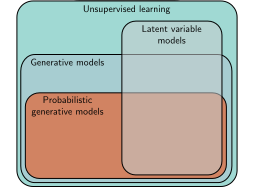
\includegraphics[width=0.7\linewidth]{png/chapter14/UnsupOverview.png}
\caption{Figure14.1}
\end{figure}

`图 14.1 无监督学习模型分类。无监督学习指在无标签数据集上训练的模型。生成模型能够合成具有与训练数据相似统计特性的新示例。其中的一个子集是基于概率的,定义了一个覆盖数据的分布。我们通过从这个分布中抽样来生成新示例。潜在变量模型(latent variable models)建立了底层解释性(latent)变量与数据之间的映射关系,这些模型可以属于以上任何一类。`

\begin{figure}[ht!]
\centering
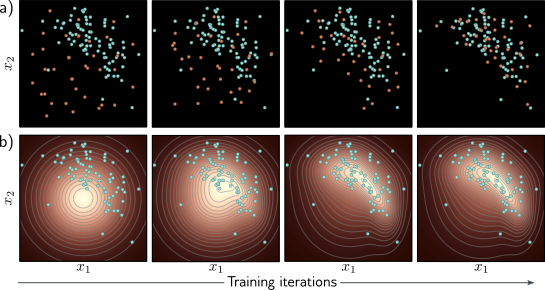
\includegraphics[width=0.7\linewidth]{png/chapter14/UnsupLearning.png}
\caption{Figure14.2}
\end{figure}

`图 14.2 拟合生成模型 a)生成对抗网络(GANs)提供了一种生成样本(橙色点)的机制。随着训练进程(从左至右),损失函数促使这些样本逐渐与真实示例(青色点)难以区分。b)概率模型(包括变分自编码器(VAEs)、规范化流(Normalizing Flows)和扩散模型(Diffusion Models))学习了训练数据上的概率分布。随着训练进程(从左至右),这个分布下真实示例的似然性增加,可以用来抽取新样本和评估新数据点的概率。`

\section{如何定义一个优秀的生成模型?}
基于潜变量的生成模型应具备以下特性:
- \textbf{高效抽样}:生成模型样本的过程在计算上应低成本,能够充分发挥现代硬件并行处理的优势。
- \textbf{高品质抽样}:生成的样本应当与模型训练所用的真实数据难以区分。
- \textbf{全面覆盖}:生成的样本应覆盖整个训练数据的分布范围,仅仅生成一小部分训练样本的相似项是不足够的。
- \textbf{良好的潜空间表现}:每一个潜变量 z 都应对应一个可信的数据示例 x。z 的平滑变动应引发 x 的平滑变化。
- \textbf{可解释的潜空间}:调整 z 的任意一个维度都应该对应于数据某个可解释特征的变化。比如,在语言模型中,可能是改变话题、时态或是文本的详略程度。
- \textbf{高效的概率计算}:如果模型基于概率,我们希望能够高效准确地计算新样本的概率。

由此,我们不禁会问:我们当前考虑的生成模型能否满足这些特性呢?虽然答案比较主观,图 14.3 对此提供了一些指导。尽管具体的归类可能存在争议,但大多数实践者认为,没有任何一个模型能够完全满足上述所有条件。

![Figure14.3](figures/chapter14/f143.png)

`图 14.3 四种生成模型的属性。生成对抗网络(GANs)、变分自编码器(VAEs)、规范化流(Flows)以及扩散模型(Diffusion Models)都不完全具备理想属性的全集。`
\section{性能量化}
前一节我们讨论了生成模型所期望具备的属性。接下来,我们将探讨对生成模型成功度量的量化标准。许多生成模型的实验选择了图像作为研究对象,这一选择主要得益于图像数据的广泛可得性及其便于定性评价的特点。据此,一些评价指标专门针对图像数据设计。

测试似然度:评估概率模型的一种方法是通过测试数据集的似然度进行比较。因为模型可能对每个训练数据点分配极高的概率,而在这些点之间分配极低的概率,所以仅通过训练数据的似然度来评估是不准确的。这样的模型虽然在训练集上似然度很高,但却只能重现训练数据。测试似然度能够反映模型从训练数据中泛化的能力,以及其覆盖范围;如果模型只给训练数据的一个子集分配了高概率,那么它在其他部分必然分配了较低的概率,这意味着部分测试样本的概率会很低。

虽然测试似然度是评价概率模型的一个合理方式,但遗憾的是,它不适用于生成对抗模型(Generative Adversarial Models,GAM)(这类模型不分配概率),并且对于变分自编码器和扩散模型来说,估计成本高昂(尽管可以计算对数似然的下界)。规范化流(Normalizing Flows)是唯一可以准确且高效计算似然度的模型类型。

\textbf{Inception 分数}:Inception 分数(IS)专为图像设计,最理想的应用场景是在 ImageNet 数据库上训练的生成模型。该分数通过一个预训练的分类模型来计算,通常是“ Inception”模型,因此而得名。它基于两个准则:首先,每个生成的图像 \(x^*\) 应当仅对应 ImageNet 数据库中的一个类别 y。因此,概率分布 \(Pr(y_i|x^*_i)\) 在正确类别上应高度集中。其次,所有生成的图像集应该等概率地被分配到各个类别中,因此平均下来,Pr(y) 应当是平坦的。

Inception 分数衡量了生成集上这两个分布间平均距离。如果一个分布高度集中而另一个分布平坦,这个距离会很大(图 14.4)。更具体地,它返回 \(Pr(y_i|x^*_i)\) 与 Pr(y) 之间期望 KL 散度的指数:

\[
IS = \exp \left( \frac{1}{I} \sum_{i=1}^{I} D_{KL} [ Pr(y|x_i^*) || Pr(y) ] \right),
\]

其中 *I* 表示生成样例的数量,且有:

\[
Pr(y) = \frac{1}{I} \sum_{i=1}^{I} Pr(y|x_i^*)。
\]

此度量标准仅适用于 ImageNet 数据库的生成模型,对特定的分类模型较为敏感;重训练这个模型可能会导致不同的数值结果。此外,它不奖励类别内部的多样性;如果模型仅生成每个类别的一个逼真示例,它就会返回一个高值。

\textbf{Fréchet Inception 距离}:此度量标准也是为图像而设计,用于计算生成样本与真实样本分布之间的对称距离。鉴于很难具体描述任一分布(实际上,描述真实样本分布正是生成模型的初衷),这个距离必须是近似的。因此,Fréchet Inception 距离通过多变量高斯分布来近似这两个分布,并利用 Fréchet 距离来估计它们之间的距离。

然而,这一度量不是基于原始数据,而是基于 Inception 分类网络中最深层激活的距离。这些隐藏单元与对象类别高度相关,因此比较发生在语义层面,而忽略了图像的更细节特征。这个度量标准虽然考虑了类别内的多样性,但极度依赖于 Inception 网络中保留的特征信息;网络丢弃的任何信息都不会影响结果。网络丢弃的部分信息可能对生成逼真样本仍然十分重要。

\textbf{流形精确度/召回率}:Fréchet Inception 距离对样本的逼真度和多样性都敏感,但不能区分这些要素。为了分离这些属性,我们考量了数据流形(即,真实样本所处的数据空间子集)与模型流形(即,生成样本所在的位置)之间的重合程度。精确度是落入数据流形内的模型样本比例,衡量了生成样本的逼真度。召回率是落入模型流形内的数据样本比例,衡量了模型能生成的真实数据的比例(图 14.5)。

为估计流形,我们在每个数据样本周围放置一个以第k近邻距离为半径的超球体。这些球体的并集近似表示了流形,可以轻易判断新点是否位于其中。这个流形也通常在分类器的特征空间中计算,这既是其优点也是缺点。

\begin{figure}[ht!]
\centering
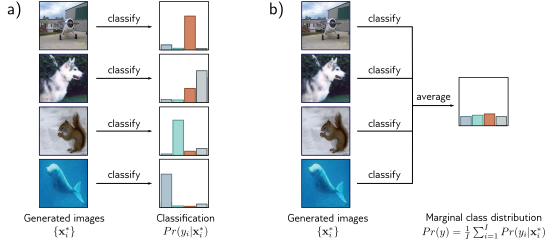
\includegraphics[width=0.7\linewidth]{png/chapter14/UnsupInception.png}
\caption{Figure14.4}
\end{figure}

`图 14.4 Inception 分数。a)一个预训练网络对生成图像进行分类。如果图像逼真,那么相应的类别概率 \(Pr(y_i | x^*_i)\) 应在正确的类别上高度集中。b)如果模型等概率地生成所有类别,边际(平均)类别概率应为平坦。Inception 分数测量了 (a) 和 (b) 中分布之间的平均距离。图片来源:Deng 等(2009)。`

\begin{figure}[ht!]
\centering
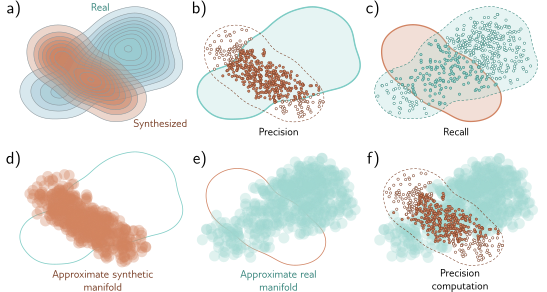
\includegraphics[width=0.7\linewidth]{png/chapter14/UnsupPrecisionRecall.png}
\caption{Figure14.5}
\end{figure}

`图 14.5 流形精确度/召回率。a)真实示例与生成模型合成样本的真实分布。b)重叠可以通过精确度(与真实示例的分布或流形重叠的合成样本的比例)和 c)召回率(与合成样本的流形重叠的真实示例的比例)来概括。d)通过取一组围绕每个样本中心的超球体的并集,可以近似合成样本的流形。这里,这些球体有固定的半径,但通常基于到第 k 近邻的距离确定半径。e)真实示例的流形也通过类似方法近似。f)精确度可计算为位于样本近似流形内的真实示例的比例。同样,召回率计算为位于真实示例近似流形内的样本的比例(未展示)。根据 Kynkäänniemi 等(2019)改编。`
\section{总结}
无监督模型能够在缺少标签的情况下掌握数据集的结构。这些模型中的一部分具有生成性,能够创造新的数据示例。再进一步,其中的一些模型是基于概率的,不仅能生成新的示例,还能对观测到的数据赋予概率。接下来四章将讨论的模型以一个已知分布的潜在变量 z 作为起点。随后,一个深度神经网络将潜在变量映射到观察到的数据空间。我们探讨了生成模型所期望的属性,并介绍了旨在量化其性能的度量指标。

\section{Notes}
热门的生成模型包括生成对抗网络(Generative Adversarial Networks, GANs, Goodfellow 等,2014)、变分自编码器(Variational Autoencoders, VAEs, Kingma \& Welling,2014)、规范化流(Normalizing Flows, Rezende \& Mohamed,2015)、扩散模型(Diffusion Models, Sohl-Dickstein 等,2015; Ho 等,2020)、自回归模型(Autoregressive Models, Bengio 等,2000; Van den Oord 等,2016b)以及基于能量的模型(Energy-Based Models, LeCun 等,2006)。除能量模型外,本书讨论了所有这些模型。Bond-Taylor 等(2022)提供了关于生成模型的最新综述。

\textbf{评估}:Salimans 等(2016)提出了 Inception 分数,而 Heusel 等(2017)提出了 Fréchet Inception 距离,两者均基于 Inception V3 模型的 Pool-3 层(Szegedy 等,2016)。Nash 等(2021)采用了该网络更早的层级,这些层级保留了更多空间信息,确保图像的空间统计特征得到复制。Kynkäänniemi 等(2019)引入了流形精度/召回方法。Barratt \& Sharma(2018)对 Inception 分数进行了详细讨论并指出其缺陷。Borji(2022)讨论了评估生成模型不同方法的优点和缺点。
